\documentclass[12pt]{article}
\usepackage{graphicx}
\usepackage{placeins}


% acronyms for text or math mode
\newcommand {\ccast} {\mbox{\small CCAST}}
\newcommand {\cris} {\mbox{\small CrIS}}

\newcommand {\airs} {\mbox{\small AIRS}}
\newcommand {\iasi} {\mbox{\small IASI}}
\newcommand {\idps} {\mbox{\small IDPS}}
\newcommand {\nasa} {\mbox{\small NASA}}
\newcommand {\noaa} {\mbox{\small NOAA}}
\newcommand {\nstar} {\mbox{\small STAR}}
\newcommand {\umbc} {\mbox{\small UMBC}}
\newcommand {\uw}   {\mbox{\small UW}}

\newcommand {\fft}  {\mbox{\small FFT}}
\newcommand {\ifft} {\mbox{\small IFFT}}
\newcommand {\fir}  {\mbox{\small FIR}}
\newcommand {\fov}  {\mbox{\small FOV}}
\newcommand {\for}  {\mbox{\small FOR}}
\newcommand {\ict}  {\mbox{\small ICT}}
\newcommand {\ils}  {\mbox{\small ILS}}
\newcommand {\igm}  {\mbox{\small IGM}}
\newcommand {\opd}  {\mbox{\small OPD}}
\newcommand {\rms}  {\mbox{\small RMS}}
\newcommand {\zpd}  {\mbox{\small ZPD}}
\newcommand {\ppm}  {\mbox{\small PPM}}
\newcommand {\srf}  {\mbox{\small SRF}}
\newcommand {\sdr}  {\mbox{\small SDR}}

\newcommand {\ES} {\mbox{\small ES}}
\newcommand {\SP} {\mbox{\small SP}}
\newcommand {\IT} {\mbox{\small IT}}
\newcommand {\SA} {\mbox{\small SA}}

\newcommand {\ET} {\mbox{\small ET}}
\newcommand {\FT} {\mbox{\small FT}}

% abbreviations, mainly for math mode
\newcommand {\real} {\mbox{real}}
\newcommand {\imag} {\mbox{imag}}
\newcommand {\atan} {\mbox{atan}}
\newcommand {\obs}  {\mbox{obs}}
\newcommand {\calc} {\mbox{calc}}
\newcommand {\sinc} {\mbox{sinc}}
\newcommand {\psinc} {\mbox{psinc}}
\newcommand {\std} {\mbox{std}}

% symbols, for math mode only
\newcommand {\wnum} {\mbox{cm$^{-1}$}}
\newcommand {\lmax} {L_{\mbox{\tiny max}}}
\newcommand {\vmax} {V_{\mbox{\tiny max}}}

\newcommand {\tauobs} {\tau_{\mbox{\tiny obs}}}
\newcommand {\taucal} {\tau_{\mbox{\tiny calc}}}
\newcommand {\Vdc}  {V_{\mbox{\tiny DC}}}

\newcommand {\rIT} {r_{\mbox{\tiny\textsc{ict}}}}
\newcommand {\rES} {r_{\mbox{\tiny\textsc{es}}}}
\newcommand {\robs} {r_{\mbox{\tiny obs}}}

\newcommand {\rITobs} {r_{\mbox{\tiny\textsc{ict}}}^{\mbox{\tiny obs}}}
\newcommand {\rITcal} {r_{\mbox{\tiny\textsc{ict}}}^{\mbox{\tiny cal}}}

\newcommand {\ITmean} {\langle\mbox{\small IT}\rangle}
\newcommand {\SPmean} {\langle\mbox{\small SP}\rangle}


\title{Progress Report \\
  Oct--Dec 2014}
\author{L.~L.~Strow \& H.~E.~Motteler \\
  \\
  UMBC Atmospheric Spectroscopy Lab \\
  Joint Center for Earth Systems Technology \\
}
\date{\today}
\begin{document}

\maketitle

\section{CrIS TVAC}

The \cris\ TVAC gas cell tests showed generally good agreement
between observed and calculated spectra.  We show representative
results from the PFL side 1 CO, CH$_4$, CO$_2$, and the MN side 1
NH$_3$ test, and a representative summary of CO and CO$_2$ residuals
across different test stages.  The PFL tests show good agreement
with calculated transmittances for CO, CH$_4$ and CO$_2$.  The CO
CH$_4$, and CO$_2$ side 1 residuals are reasonably consistent across
the MN, PFH, and PFL tests.  There was a low-frequency component in
the residuals in some tests.  In addition, there was a significant
difference between nominal and observed gas cell pressure in some
tests.  When this occured the observed value was used for the
calculated spectra.

There is a close parallel between our expression for
transmittance
    \[\tauobs = f\cdot\SA^{-1}\cdot f \cdot \frac{\FT_2 - \FT_1}{\ET_2 - \ET_1}\]
and our default \cris\ calibration equation
    \[r_{\mbox{\tiny obs}} = F \cdot r_{\mbox{\tiny ICT}}\cdot f \cdot
    \SA^{-1}\cdot f \cdot \frac{\ES - \SP}{\IT - \SP} \]
Here $f$ is a raised-cosine bandpass filter, $\SA^{-1}$ the inverse
of the ILS matrix, $r_{\mbox{\tiny ICT}}$ is expected ICT radiance
at the sensor grid, and $F$ is Fourier interpolation from sensor to
user grid.  The same $f$ is applied to line-by-line transmittances
before convolution to the \cris\ sensor grid.   All tests shown here
were done using UMBC LBL for calculated transmittances.

To match observed and calculated transmittance spectra we minimize
$\rms(a\cdot\tauobs + b - \taucal)$ over the fitting interval as a
function of the metrology laser wavelength.  From this we get both a
conventional residual and the difference of wavelength at the minima
from the neon calibration value.  The latter difference is the
``metrology laser residual.''  The CO and CH$_4$ side 1 residuals
are very consistent across the MN, PFH, and PFL tests.  For CO$_2$,
the MN and PFH tests were in good agreement, in comparison with the
PFL tests.  Our NH$_3$ residuals were generally larger than for
CO$_2$.

Remaining work includes checking and refining measurements of the
focal plane geometery and adding a nonlinearity correction to the
observed data.

\newpage

%----------- slide --------------------------------------------------%
% \frametitle{CO obs and calc}

\begin{figure}
  \centering
  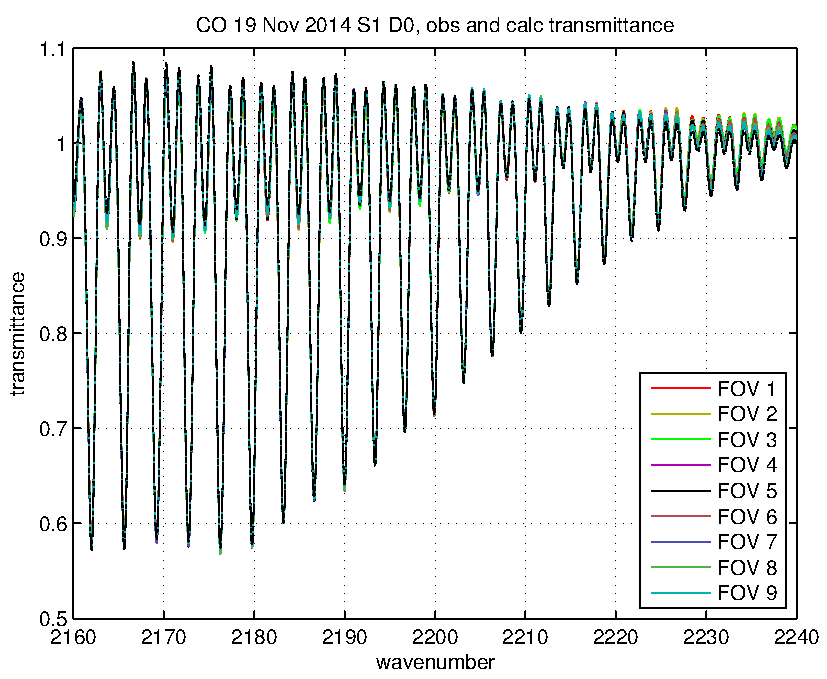
\includegraphics[height=8cm]{figures/CO_obs_and_calc.pdf}
  \caption{CO observed and calculated transmittance for all {\fov}s,
    over the fitting interval.  At this level of detail we see all
    values are very close.}
\end{figure}

%----------- slide --------------------------------------------------%
% \frametitle{CO obs minus calc}

\begin{figure}
  \centering
  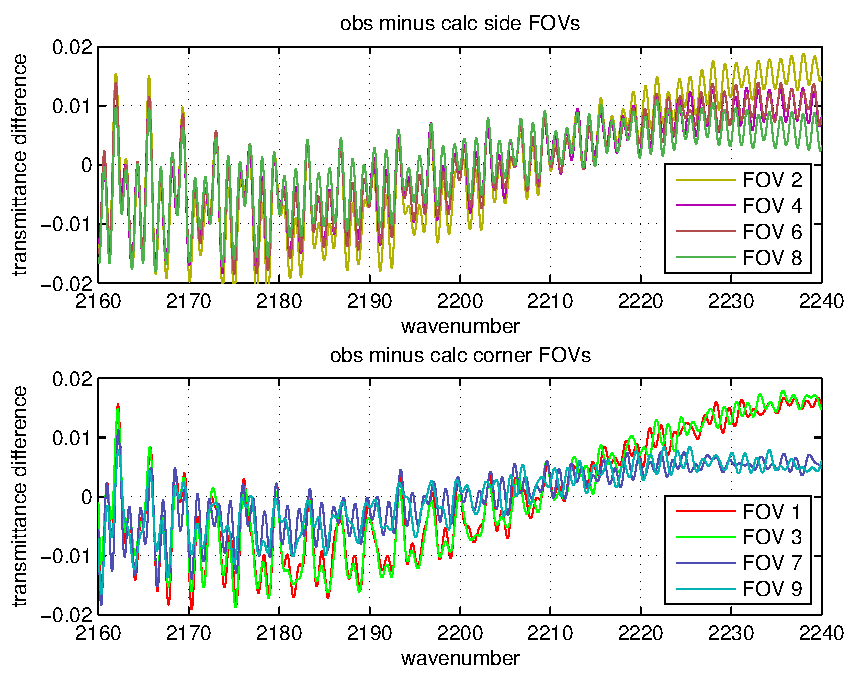
\includegraphics[height=8cm]{figures/CO_breakout_2.pdf}
  \caption{CO observed minus calculated transmittance for side and
    corner FOVs, over the fitting interval.}
\end{figure}

%----------- slide --------------------------------------------------%
% \frametitle{CH$_4$ obs and calc}

\begin{figure}
  \centering
  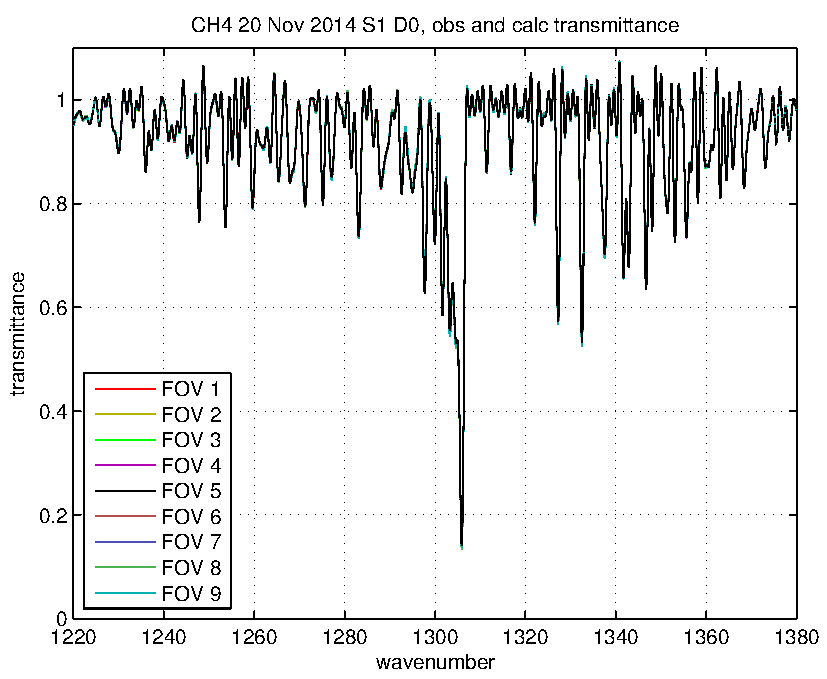
\includegraphics[height=8cm]{figures/CH4_obs_and_calc.pdf}
  \caption{CH$_4$ observed and calculated transmittance for all
    {\fov}s, over the fitting interval.  At this level of detail we see
    all values are very close.}
\end{figure}

%----------- slide --------------------------------------------------%
% \frametitle{CH$_4$ obs minus calc}

\begin{figure}
  \centering
  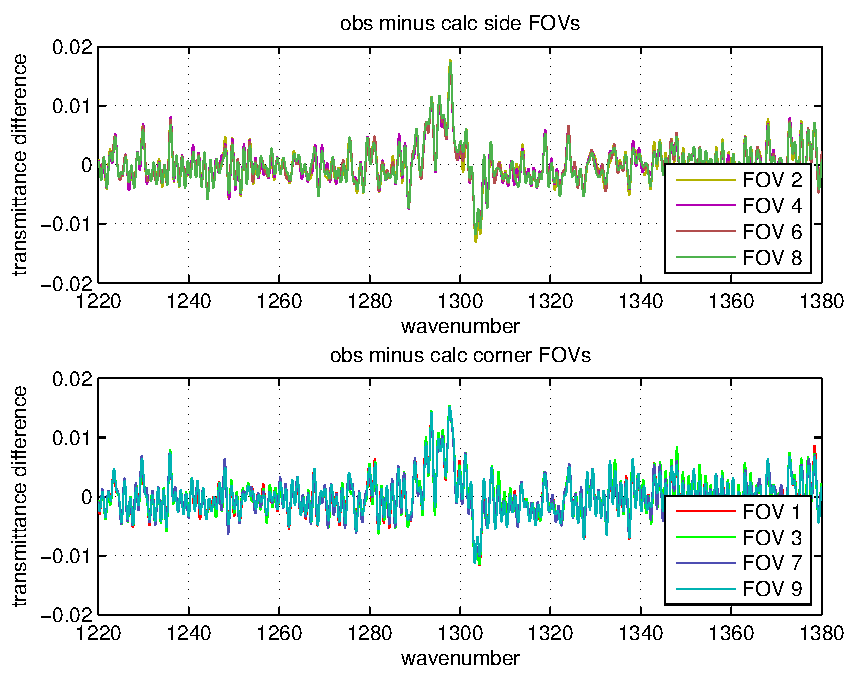
\includegraphics[height=8cm]{figures/CH4_breakout_2.pdf}
  \caption{CH$_4$ observed minus calculated transmittance for side
    and corner {\fov}s, over the fitting interval.}
\end{figure}

%----------- slide --------------------------------------------------%
% \frametitle{NH$_3$ obs and calc}

\begin{figure}
  \centering
  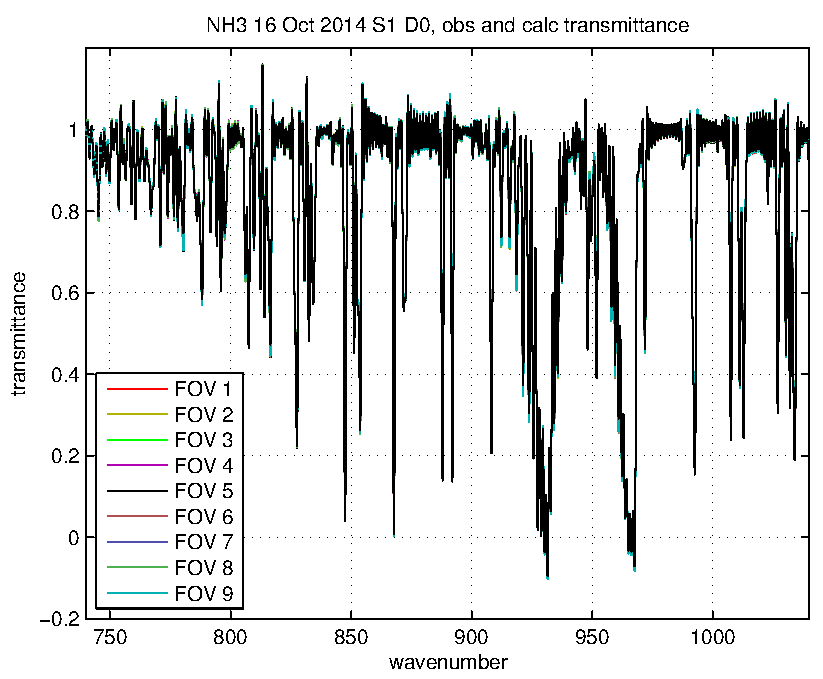
\includegraphics[height=8cm]{figures/NH3_obs_and_calc.pdf}
  \caption{NH$_3$ observed and calculated transmittance for all
    {\fov}s, over the fitting interval.  At this level of detail we
    see all values are close.}
\end{figure}

%----------- slide --------------------------------------------------%
% \frametitle{NH$_3$ obs minus calc}

\begin{figure}
  \centering
  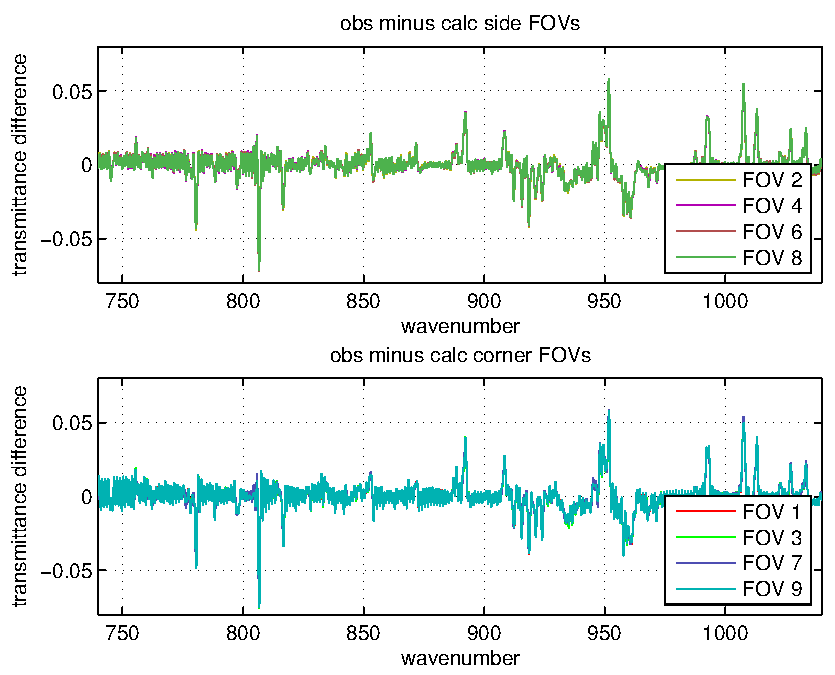
\includegraphics[height=8cm]{figures/NH3_breakout_2.pdf}
  \caption{NH$_3$ observed minus calculated transmittance for side
    and corner {\fov}s, over the fitting interval.}
\end{figure}

%----------- slide --------------------------------------------------%
% \frametitle{CO$_2$ obs and calc}

\begin{figure}
  \centering
  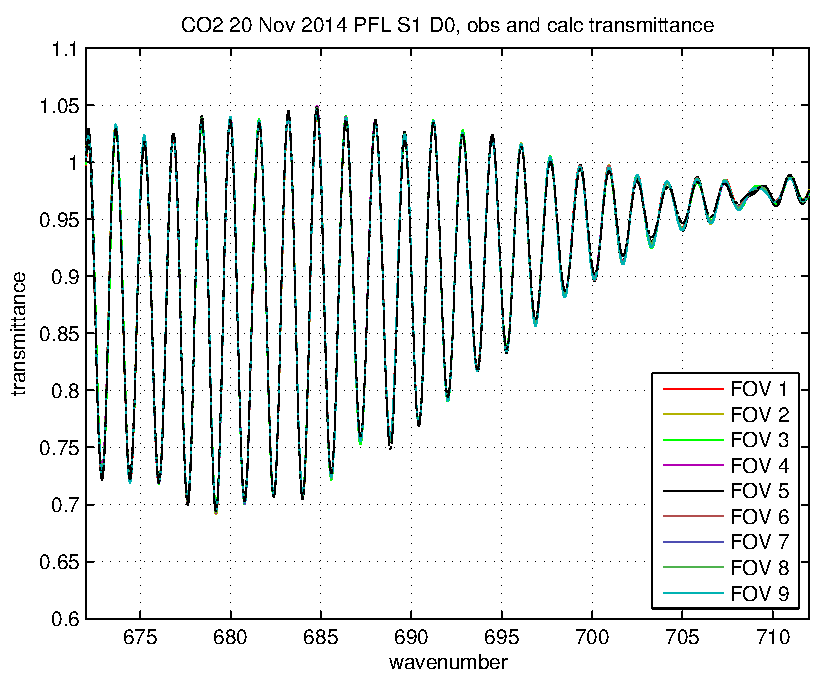
\includegraphics[height=8cm]{figures/CO2_obs_and_calc.pdf}
  \caption{CO$_2$ observed and calculated transmittance for all
    {\fov}s, over the fitting interval.  At this level of detail we
    see all values are close.}
\end{figure}

%----------- slide --------------------------------------------------%
% \frametitle{CO$_2$ obs minus calc}

\begin{figure}
  \centering
  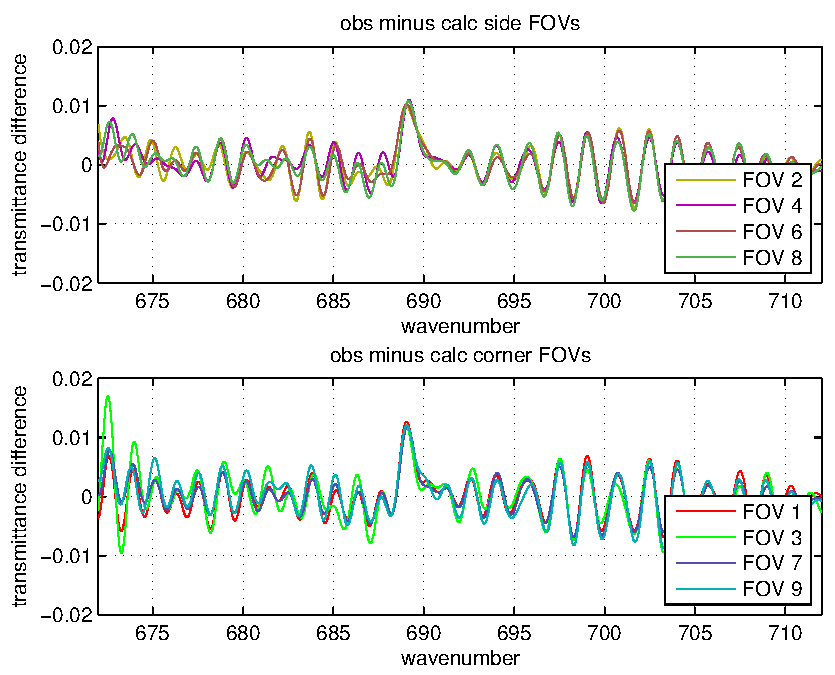
\includegraphics[height=8cm]{figures/CO2_breakout_2.pdf}
  \caption{CO$_2$ observed minus calculated transmittance for side
    and corner {\fov}s, over the fitting interval.}
\end{figure}

%----------- slide --------------------------------------------------%
% \frametitle{CO side 1 test comparison}

\begin{figure}
\begin{verbatim}
          --- rms fit ----        --- met laser --
  FOV    MN      PH      PL      MN      PH      PL  
   1     4.4     1.5     9.9    13.2    15.0    10.3
   2     2.8     3.5    10.6     3.4     5.2     2.3
   3     4.9     2.4    10.0     4.1     2.8     2.6
   4     2.7     3.4     7.7     4.4     6.7     3.9
   5     1.7     2.8     7.9     3.1     3.1     2.6
   6     2.4     3.3     8.1     3.1     2.6     3.6
   7     3.9     1.6     5.3    -0.5    -0.5    -0.8
   8     2.4     3.3     6.5    -6.7    -6.7    -5.7
   9     4.7     2.6     5.2     7.2     4.9     7.5

  log torr: MN 40.5 PH 39.9 PL 45.0
  obs torr: MN 41.0 PH 26.0 PL 45.0
\end{verbatim}
\caption{CO side 1 test comparison.  ``rms fit'' is $1000 \cdot
  \rms(a\cdot\tauobs + b - \taucal)$ and ``met laser'' is the
  metrology laser residual.}
\end{figure}

%----------- slide --------------------------------------------------%
% \frametitle{CO$_2$ side 1 test comparison}

\begin{figure}
\begin{verbatim}
          --- rms fit ----        --- met laser --
  FOV    MN      PH      PL      MN      PH      PL  
   1     1.6     1.4     3.3     8.3    11.3     0.3
   2     1.6     1.2     3.2     2.1     2.6    -6.2
   3     2.8     1.9     4.0     1.3    -0.3    -4.1
   4     1.8     1.8     3.0     3.6     5.4    -3.1
   5     2.5     2.1     3.4     3.6     4.9    -1.8
   6     2.5     1.6     3.0     2.1     1.8    -3.9
   7     1.7     1.2     3.1    -6.2    -3.9   -13.4
   8     1.8     2.4     3.1    -6.5    -4.9   -11.1
   9     1.7     1.9     3.6     0.8     0.8    -6.2

log torr: MN 40.2 PH 40.0 PL 40.7
obs torr: MN 40.2 PH 40.0 PL 22.0
\end{verbatim}
\caption{CO$_2$ side 1 test comparison.  ``rms fit'' is $1000 \cdot
    \rms(a\cdot\tauobs + b - \taucal)$ and ``met laser'' is the
    metrology laser residual}
\end{figure}

\FloatBarrier

%----------- slide --------------------------------------------------%
\section{CrIS full resolution processing}

After several earlier tests, on 4 Dec 2014 the CrIS instrument
changed over to full resolution processing, with a nominal 0.8 cm
OPD for all three bands.  We show a representative comparison of
results from the {\umbc} {\ccast} and \noaa/{\nstar} full resolution
processing.  The tests shown here were done with {\ccast} and
{\noaa} high res data from 6--8 Dec 2014.  We take the average and
standard deviation of \for\ 15 and 16 independently for each \fov,
and compare these values with the values for \fov\ 5.  Results are
for 32,186 \ccast\ and 32,120 {\noaa} descending {\for}s.  The
intent is to show variation among {\fov}s, as might arise from
varying nonlinearity or artifacts of the self-apodization correction.
Due to some initial problems with the impulse mask, as a precaution
{\for}s where any LW channel was greater than 320K were discarded.

For the MW band \fov\ 7 is the least linear, and only partially
corrected with the {\ccast} first-order adjustment.  The {\noaa}
variation in {\fov} response is much greater than what we see with
{\ccast}.  This may be due to problems with the \noaa\ nonlinearity
correction.  A normalized frequency domain representation of the
numeric filter needs a scaling factor to match the original
nonlinearity measurements.  We used 1.6047 for LW, 0.9826 for MW,
and 0.2046 for SW for these values.

For the SW band \ccast\ and \noaa\ are generally in good agreement.
Residuals for both are significantly larger than for the LW band,
and \noaa\ vs \ccast\ differences are generally greatest for the
coldest lines and regions.  \fov\ 7 minus \fov\ 5 is significantly
greater than for other \fov s at 2255 and 2359 \wnum, for both
\ccast\ and \noaa.

There is significant convergence in the \ccast\ and
\noaa\ processing.  We are working with Yong Han's group on the MW
differences.  Variation due to nonlinearity, especially for the MW
band, is significantly greater than some of the more subtle effects
we have been considering recently.  Note again that these results
are relative to \fov\ 5 and are not comparisons with with expected
observed radiance from model data or radiance from other sounders.

%----------- slide --------------------------------------------------%
% \frametitle{ccast MW mean}

\begin{figure}
  \centering
  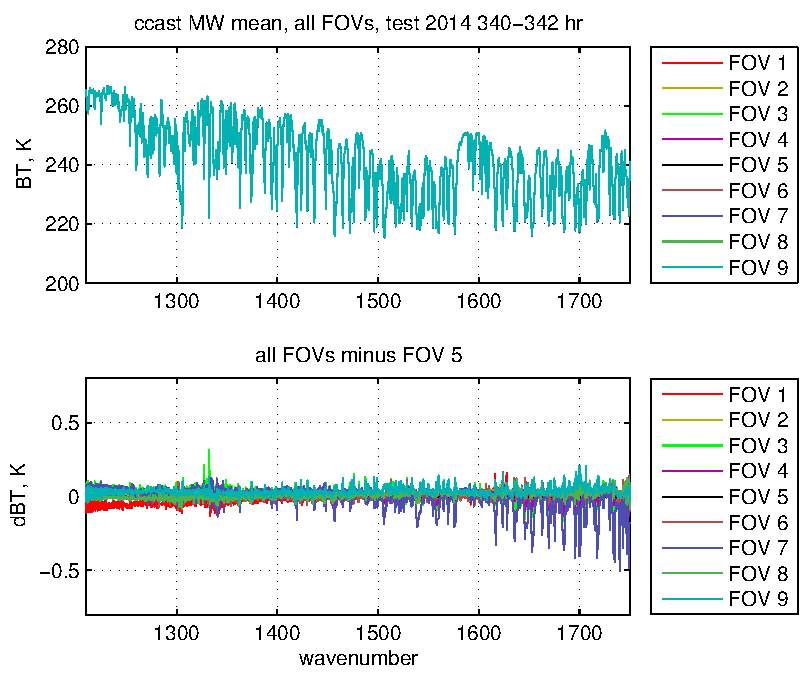
\includegraphics[height=8cm]{figures/ccast_MW_avg_2014_340-342_hr.pdf}
  \caption{\ccast\ MW mean}
\end{figure}  

%----------- slide --------------------------------------------------%
% \frametitle{noaa MW mean}

\begin{figure}
  \centering
  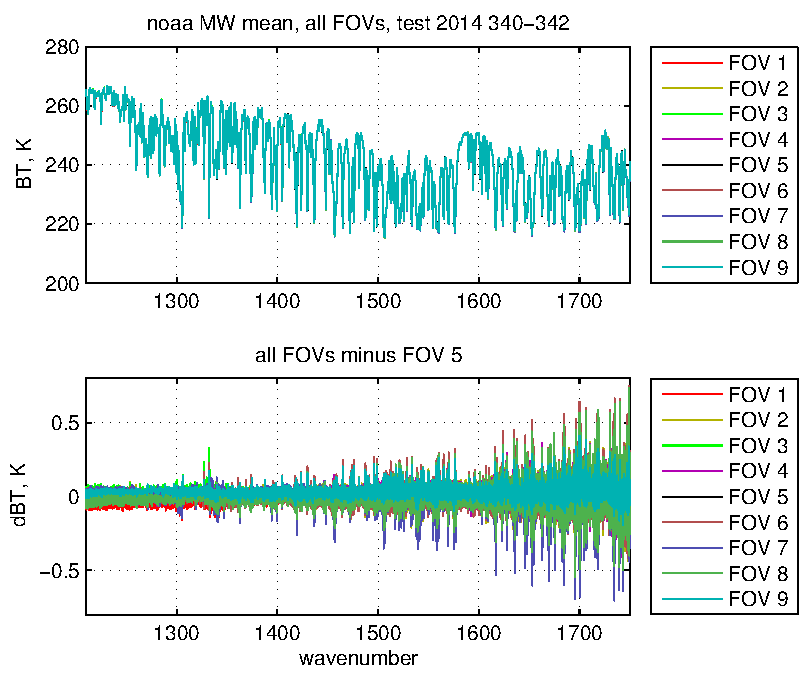
\includegraphics[height=8cm]{figures/noaa_MW_avg_2014_340-342.pdf}
  \caption{\noaa\ MW mean}
\end{figure}

%----------- slide --------------------------------------------------%
% \frametitle{ccast MW fov groups}

\begin{figure}
  \centering
  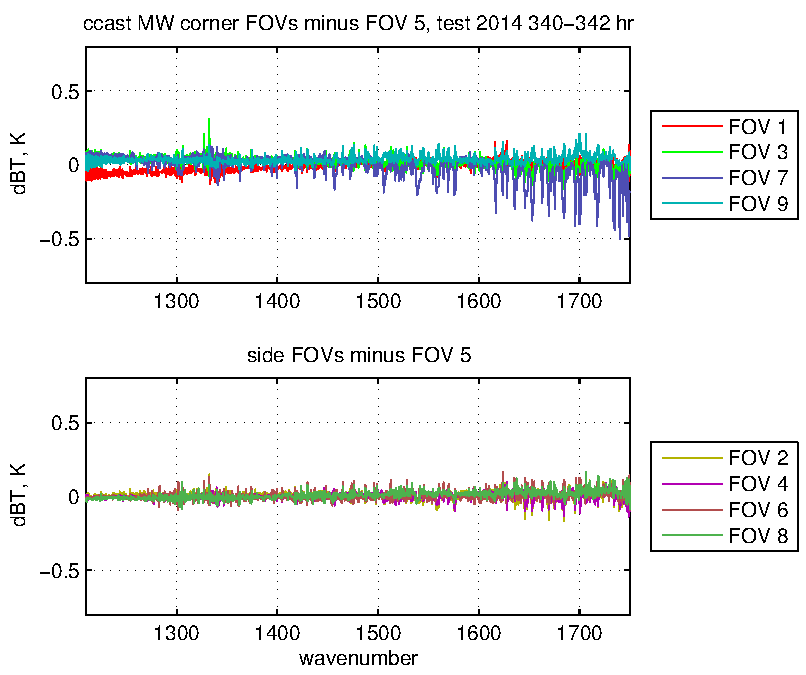
\includegraphics[height=8cm]{figures/ccast_MW_dif_2014_340-342_hr.pdf}
  \caption{\ccast\ MW \fov\ groups}
\end{figure}

%----------- slide --------------------------------------------------%
% \frametitle{noaa MW fov groups}

\begin{figure}
  \centering
  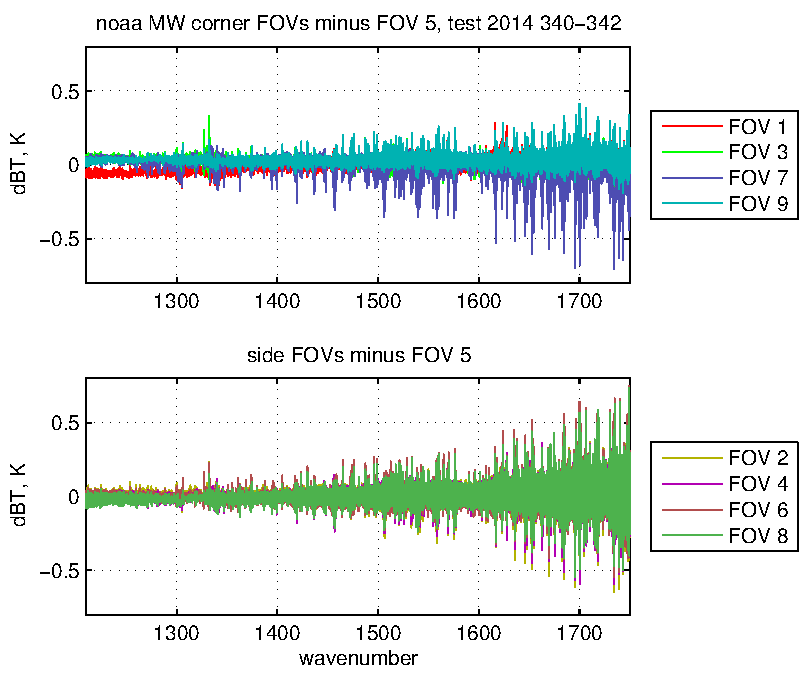
\includegraphics[height=8cm]{figures/noaa_MW_dif_2014_340-342.pdf}
  \caption{\noaa\ MW \fov\ groups}
\end{figure}


%----------- slide --------------------------------------------------%
% \frametitle{ccast SW mean}

\begin{figure}
  \centering
  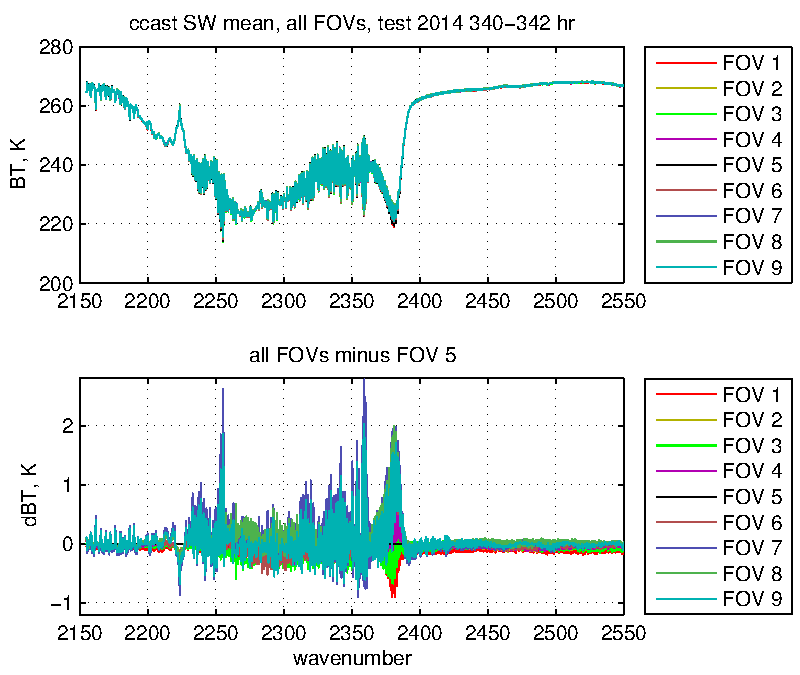
\includegraphics[height=8cm]{figures/ccast_SW_avg_2014_340-342_hr.pdf}
  \caption{\ccast\ SW mean}
\end{figure}

%----------- slide --------------------------------------------------%
% \frametitle{noaa SW mean}

\begin{figure}
  \centering
  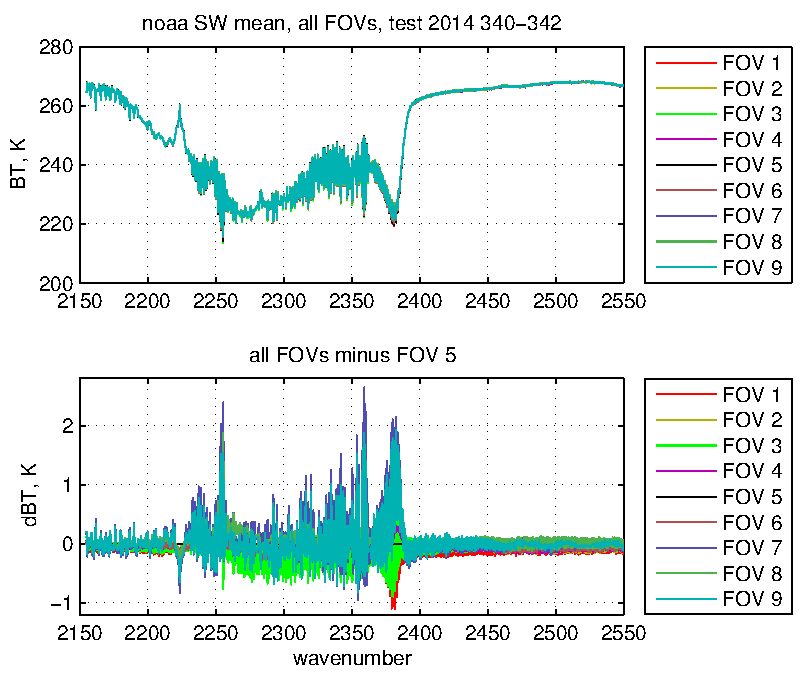
\includegraphics[height=8cm]{figures/noaa_SW_avg_2014_340-342.pdf}
  \caption{\noaa\ SW mean}
\end{figure}


%----------- slide --------------------------------------------------%
% \frametitle{ccast SW fov groups}

\begin{figure}
  \centering
  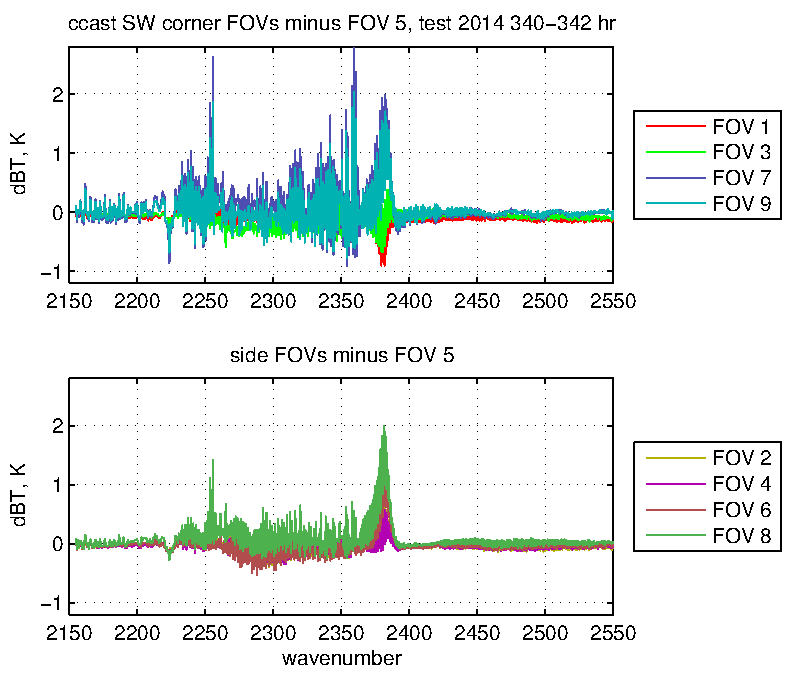
\includegraphics[height=8cm]{figures/ccast_SW_dif_2014_340-342_hr.pdf}
  \caption{\ccast\ SW \fov\ groups}
\end{figure}

%----------- slide --------------------------------------------------%
% \frametitle{noaa SW fov groups}

\begin{figure}
  \centering
  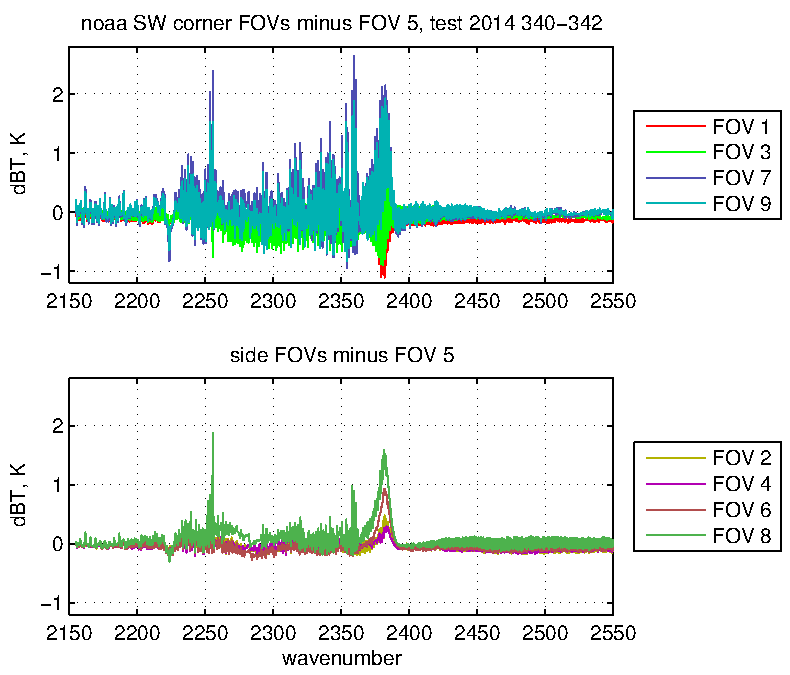
\includegraphics[height=8cm]{figures/noaa_SW_dif_2014_340-342.pdf}
  \caption{\noaa\ SW \fov\ groups}
\end{figure}

%----------- slide --------------------------------------------------%
\end{document}
